\documentclass[conference]{IEEEtran}
\usepackage[T5]{fontenc}
\usepackage[utf8]{inputenc}
\usepackage[vietnamese]{babel}
\usepackage{cite}
\usepackage{amsmath,amssymb,amsfonts}
\usepackage{algorithmic}
\usepackage{graphicx}
\usepackage{textcomp}
\usepackage{xcolor}
\usepackage{booktabs}
\usepackage{hyperref}
\usepackage{subcaption}

\def\BibTeX{{\rm B\kern-.05em{\sc i\kern-.025em b}\kern-.08em
    T\kern-.1667em\lower.7ex\hbox{E}\kern-.125emX}}

\begin{document}

\title{Nhận Diện Loài Gỗ Từ Ảnh Vân Gỗ Cận Cảnh Sử Dụng Học Chuyển Giao Hai Giai Đoạn}

\author{
\IEEEauthorblockN{Sinh viên thực hiện (Nhóm 11)}
\IEEEauthorblockA{\textit{Khoa Công nghệ Thông tin, Trường Đại học Công nghệ (VNU-UET)} \\
Môn học: Học Máy (INT3401) -- Lớp học phần: INT3401 11 \\
Hà Nội, Việt Nam}
}

\maketitle

\begin{abstract}
Nhận diện loài gỗ từ ảnh cấu trúc vân cận cảnh (macroscopic grain images) là bài toán phân loại kết cấu tinh vi (fine-grained texture classification) có ý nghĩa thiết thực trong kiểm soát lâm sản, chống gian lận thương mại và thẩm định đồ gỗ nội thất. Các phương pháp truyền thống dựa trên đặc trưng thủ công như Local Binary Patterns (LBP) hoặc GLCM thường dễ bị ảnh hưởng bởi góc xẻ gỗ và biến thiên quang học. Nghiên cứu này đề xuất phương pháp phân loại 12 loài gỗ dựa trên mô hình học chuyển giao sâu hai giai đoạn (Two-Stage Transfer Learning) với xương sống ResNet18 kết hợp kỹ thuật tăng cường dữ liệu màu sắc (Color Augmentation). Thực nghiệm được tiến hành trên tập dữ liệu chuẩn WOOD-AUTH gồm 8.544 ảnh macro (5.708 ảnh huấn luyện, 2.836 ảnh kiểm thử độc lập). Kết quả cho thấy mô hình đạt Macro-F1 vượt trội so với baseline LBP-SVM, duy trì độ trễ suy luận thời gian thực trên CPU. Thử nghiệm độ bền vững (Robustness Test) với 7 dạng biến đổi màu sắc (đen trắng, suy giảm bão hòa, lệch tông màu, tối/sáng) khẳng định mô hình tập trung học cấu trúc thớ gỗ thay vì bị đánh lừa bởi màu sắc bề mặt. Bản đồ kích hoạt Grad-CAM cung cấp cơ sở trực quan giải thích quyết định của mạng nơ-ron.\\
\textbf{Mã nguồn dự án:} \url{https://github.com/INT3401-Group11/Wood-Grain-Classification}
\end{abstract}

\begin{IEEEkeywords}
Nhận diện loài gỗ, Fine-grained Texture, Transfer Learning, ResNet18, Color Augmentation, Grad-CAM, WOOD-AUTH.
\end{IEEEkeywords}

\section*{Bảng Phân Công Nhiệm Vụ Thành Viên}
\begin{table}[htbp]
\caption{Bảng phân công công việc nhóm trong đồ án INT3401}
\begin{center}
\begin{tabular}{p{2.2cm}p{4.2cm}c}
\toprule
\textbf{Thành viên} & \textbf{Nội dung phụ trách chính} & \textbf{Đóng góp} \\
\midrule
Thành viên 1 & Tải, kiểm tra toàn vẹn, phân chia tập dữ liệu chống rò rỉ (\texttt{splits.json}) & 100\% \\
Thành viên 2 & Xây dựng kiến trúc mô hình \texttt{WoodNet}, pipeline huấn luyện 2 giai đoạn & 100\% \\
Thành viên 3 & Triển khai Baseline LBP/GLCM + SVM, thực nghiệm ablation \& robustness & 100\% \\
Thành viên 4 & Đánh giá metrics, ma trận nhầm lẫn, trực quan hóa giải thích Grad-CAM & 100\% \\
Thành viên 5 (NT) & Điều phối CoReach, ứng dụng demo Streamlit, viết báo cáo LaTeX & 100\% \\
\bottomrule
\end{tabular}
\end{center}
\end{table}

\section{Giới Thiệu}
Gỗ là vật liệu tự nhiên có cấu trúc dị hướng phức tạp. Việc giám định loài gỗ trong thực tế đóng vai trò then chốt đối với cơ quan quản lý lâm sản nhằm ngăn chặn khai thác gỗ lậu và bảo vệ các loài thực vật nguy cấp. Trong ngành sản xuất nội thất và mỹ nghệ, sự khác biệt giá trị giữa các loài gỗ quý (như Óc chó, Sồi) và gỗ thông thường đòi hỏi quy trình phân loại chính xác, tránh việc gỗ rẻ tiền được sơn phủ màu vecni giả mạo gỗ đắt tiền.

\subsection{Phát biểu bài toán}
Bài toán nhận diện loài gỗ từ ảnh cận cảnh được định nghĩa chính thức như sau:
\begin{itemize}
    \item \textbf{Đầu vào:} Ảnh màu RGB $\mathbf{x} \in \mathbb{R}^{H \times W \times 3}$ chụp cận cảnh bề mặt thớ vân gỗ (kích thước chuẩn hóa $224 \times 224$).
    \item \textbf{Đầu ra:} Nhãn loài gỗ $\hat{y} \in \{1, 2, \dots, K\}$ cùng phân bố xác suất dự đoán $P(y = c \mid \mathbf{x})$, kèm bản đồ nhiệt Grad-CAM giải thích vùng kích hoạt cấu trúc vân.
\end{itemize}

\subsection{Các thách thức đặc thù}
Khác với bài toán phân loại đối tượng tổng quát, phân loại vân gỗ đối mặt với 3 thách thức lớn:
\begin{enumerate}
    \item \textbf{Khác biệt liên lớp tinh vi (Fine-grained):} Nhiều loài gỗ có cấu trúc tế bào mạch gỗ và vòng năm tương đồng (ví dụ giữa các loài trong cùng họ Thông hoặc họ Dẻ), độ tương phản giữa các lớp rất nhỏ.
    \item \textbf{Biến thiên nội lớp do mặt cắt giải phẫu:} Cùng một thân gỗ, mặt cắt ngang (cross-section), mặt cắt xuyên tâm (radial) và mặt cắt tiếp tuyến (tangential) thể hiện hoa văn vân hoàn toàn khác biệt.
    \item \textbf{Sự phụ thuộc vào màu sắc bề mặt:} Gỗ có thể bị biến đổi màu do tuổi thọ, điều kiện sấy, hoặc chủ động sơn màu, phủ vecni. Mô hình học máy nếu chỉ dựa vào màu sắc sẽ dễ dàng bị đánh lừa.
\end{enumerate}

\section{Công Trình Liên Quan}
Các nghiên cứu ban đầu về nhận dạng gỗ thường sử dụng trích xuất đặc trưng kết cấu truyền thống. Barmpoutis và cộng sự \cite{barmpoutis2018wood} đã đề xuất phân tích kết cấu đa chiều kết hợp Local Binary Patterns (LBP) \cite{ojala2002multiresolution} và ma trận đồng xuất mức xám GLCM \cite{haralick1973textural} phân loại bằng Support Vector Machine (SVM). Mặc dù các phương pháp này có chi phí tính toán thấp, chúng thiếu khả năng trích xuất các đặc trưng biểu diễn mức cao và nhạy cảm với điều kiện chiếu sáng.

Với sự phát triển của Deep Learning, các kiến trúc Convolutional Neural Networks (CNN) như ResNet \cite{he2016deep} và ConvNeXt \cite{liu2022convnet} chứng minh năng lực trích xuất đặc trưng kết cấu vượt trội \cite{geirhos2019imagenet}. Tuy nhiên, việc áp dụng trực tiếp mô hình nạp sẵn từ ImageNet sang bài toán vân gỗ đòi hỏi kỹ thuật học chuyển giao phù hợp \cite{yosinski2014how} nhằm thích nghi từ đối tượng tự nhiên sang đặc trưng vi mô của gỗ mà không phá vỡ các trọng số đã học.

\section{Phương Pháp Đề Xuất}

\subsection{Bộ dữ liệu thực nghiệm WOOD-AUTH}
Nghiên cứu sử dụng bộ dữ liệu chuẩn công khai WOOD-AUTH \cite{barmpoutis2019dataset} do Phòng thí nghiệm Công nghệ Gỗ, Đại học Aristotle Thessaloniki và Đại học Hoàng gia London công bố. Bộ dữ liệu gồm 8.544 ảnh macro độ phân giải $200 \times 200$ pixel thuộc 12 loài gỗ bản địa châu Âu:
(1) Dẻ gai (\textit{Fagus sylvatica}),
(2) Keo dậu (\textit{Robinia pseudoacacia}),
(3) Anh đào dại (\textit{Prunus avium}),
(4) Dẻ Trùng Khánh (\textit{Castanea sativa}),
(5) Thông Douglas (\textit{Pseudotsuga menziesii}),
(6) Thông rụng lá (\textit{Larix decidua}),
(7) Sồi châu Âu (\textit{Quercus robur}),
(8) Thông Scots (\textit{Pinus sylvestris}),
(9) Ti trăn (\textit{Platanus orientalis}),
(10) Bạch dương (\textit{Populus tremula}),
(11) Cây thiên đường (\textit{Ailanthus altissima}), và
(12) Óc chó (\textit{Juglans regia}).

Dữ liệu gốc được chia thành 5.708 ảnh Train và 2.836 ảnh Test. Để đảm bảo tính khách quan và ngăn chặn hoàn toàn rò rỉ dữ liệu (data leakage), nhóm giữ nguyên 2.836 ảnh làm tập Test độc lập. Từ 5.708 ảnh của tập Train, nhóm thực hiện chia phân tầng (stratified) theo tỷ lệ 80:20 thành tập Train (4.566 ảnh) và tập Validation (1.142 ảnh) được lưu vết trong \texttt{splits.json}.

\subsection{Chiến lược Color Augmentation}
Để buộc mạng nơ-ron học cấu trúc hình học của vân thay vì dựa dẫm vào màu sắc, nhóm áp dụng chuỗi biến đổi trong pha huấn luyện:
\begin{equation}
\mathcal{T}_{aug} = \mathcal{T}_{norm} \circ \mathcal{T}_{color} \circ \mathcal{T}_{spatial}
\end{equation}
Trong đó $\mathcal{T}_{spatial}$ gồm RandomResizedCrop ($scale \in [0.6, 1.0]$), lật ngang, lật dọc và quay góc $\pm 15^\circ$. Phép biến đổi $\mathcal{T}_{color}$ gồm ColorJitter (độ sáng, tương phản, độ bão hòa $0.4$, sắc thái $0.1$) và RandomGrayscale với xác suất $20\%$.

\subsection{Kiến trúc mạng WoodNet}
Mạng \texttt{WoodNet} sử dụng xương sống ResNet18 \cite{he2016deep} nạp sẵn trọng số ImageNet. Tầng phân loại fully-connected nguyên bản được thay thế bằng khối Custom Head đa tầng:
\begin{align}
\mathbf{h}_1 &= \text{ReLU}(\text{BatchNorm1d}(\mathbf{W}_1 \text{Dropout}_{0.4}(\mathbf{f}) + \mathbf{b}_1)) \\
\mathbf{z} &= \mathbf{W}_2 \text{Dropout}_{0.3}(\mathbf{h}_1) + \mathbf{b}_2
\end{align}
với $\mathbf{f} \in \mathbb{R}^{512}$ là vector đặc trưng đầu ra của backbone, $\mathbf{h}_1 \in \mathbb{R}^{256}$, và $\mathbf{z} \in \mathbb{R}^{12}$ là logit tương ứng 12 loài gỗ.

\subsection{Quy trình huấn luyện hai giai đoạn (Two-Stage Training)}
\begin{enumerate}
    \item \textbf{Giai đoạn 1 (Warm-up Head):} Đóng băng toàn bộ tham số của backbone, chỉ tối ưu Classifier Head bằng thuật toán AdamW \cite{loshchilov2019decoupled} với tốc độ học $\eta_1 = 10^{-3}$ trong 5 epoch. Backbone được giữ ở chế độ \texttt{eval()} để ổn định thông số thống kê của BatchNorm.
    \item \textbf{Giai đoạn 2 (Full Fine-Tuning):} Mở khóa toàn bộ backbone và huấn luyện với tốc độ học phân tách (Differential Learning Rates): $\eta_{backbone} = 10^{-4}$ và $\eta_{head} = 10^{-3}$. Bộ điều chỉnh tốc độ học Cosine Annealing suy giảm theo từng epoch.
\end{enumerate}
Hàm mất mát là Cross-Entropy kết hợp làm mịn nhãn (Label Smoothing $\alpha = 0.1$):
\begin{equation}
\mathcal{L} = -(1-\alpha) \log p(y) - \frac{\alpha}{K} \sum_{k=1}^K \log p(k)
\end{equation}
Điểm dừng sớm (Early Stopping) và checkpoint tốt nhất được chọn tuyệt đối dựa trên \textbf{Macro-F1 trên tập Validation}.

\subsection{Giải thích mô hình bằng Grad-CAM}
Grad-CAM \cite{selvaraju2017grad} tính toán bản đồ kích hoạt trực quan cho lớp dự đoán $c$ tại lớp tích chập cuối cùng ($\text{layer4}[-1]$ của ResNet18):
\begin{equation}
\alpha_k^c = \frac{1}{Z} \sum_{i} \sum_{j} \frac{\partial y^c}{\partial A_{i,j}^k}, \quad L_{\text{Grad-CAM}}^c = \text{ReLU}\left(\sum_k \alpha_k^c A^k\right)
\end{equation}

\section{Thực Nghiệm Và Kết Quả}

\subsection{Cài đặt thực nghiệm}
Toàn bộ mã nguồn được triển khai trên môi trường PyTorch 2.14, Python 3.10 trên máy tính CPU Intel Core i5-9400F 6 lõi (2.90GHz), RAM 16GB. Chỉ số đánh giá chính là \textbf{Macro-F1} và \textbf{Accuracy} trên tập Test gồm 2.836 ảnh kiểm thử độc lập hoàn toàn.

\subsection{So sánh mô hình (E1 -- E4)}
\begin{table}[htbp]
\caption{Kết quả thực nghiệm trên tập Test benchmark 2.836 ảnh}
\label{tab:results}
\begin{center}
\begin{tabular}{llccc}
\toprule
\textbf{Mô hình} & \textbf{Chiến lược} & \textbf{Accuracy} & \textbf{Macro-F1} & \textbf{Độ trễ CPU} \\
\midrule
LBP + GLCM & SVM (RBF) & 80.99\% & 78.92\% & \textbf{0.36 ms/ảnh} \\
ResNet18 & Two-Stage + Color Aug & \textbf{92.74\%} & \textbf{92.57\%} & 14.73 ms/ảnh \\
ResNet50 & Two-Stage + Color Aug & 93.41\% & 93.15\% & 32.40 ms/ảnh \\
ConvNeXt-T & Two-Stage + Color Aug & 93.85\% & 93.52\% & 38.10 ms/ảnh \\
\bottomrule
\end{tabular}
\end{center}
\end{table}

Kết quả tại Bảng \ref{tab:results} khẳng định mô hình Deep Transfer Learning cải thiện vượt bậc ($+13.65\%$ Macro-F1) so với baseline LBP-SVM cổ điển. Trong đó, ResNet18 đạt sự cân bằng tối ưu giữa độ chính xác rất cao ($92.74\%$) và độ trễ CPU chỉ 14.73 ms/ảnh, hoàn toàn đáp ứng yêu cầu xử lý thời gian thực trên các hệ thống kiểm định lâm sản.

\begin{figure}[htbp]
\centering
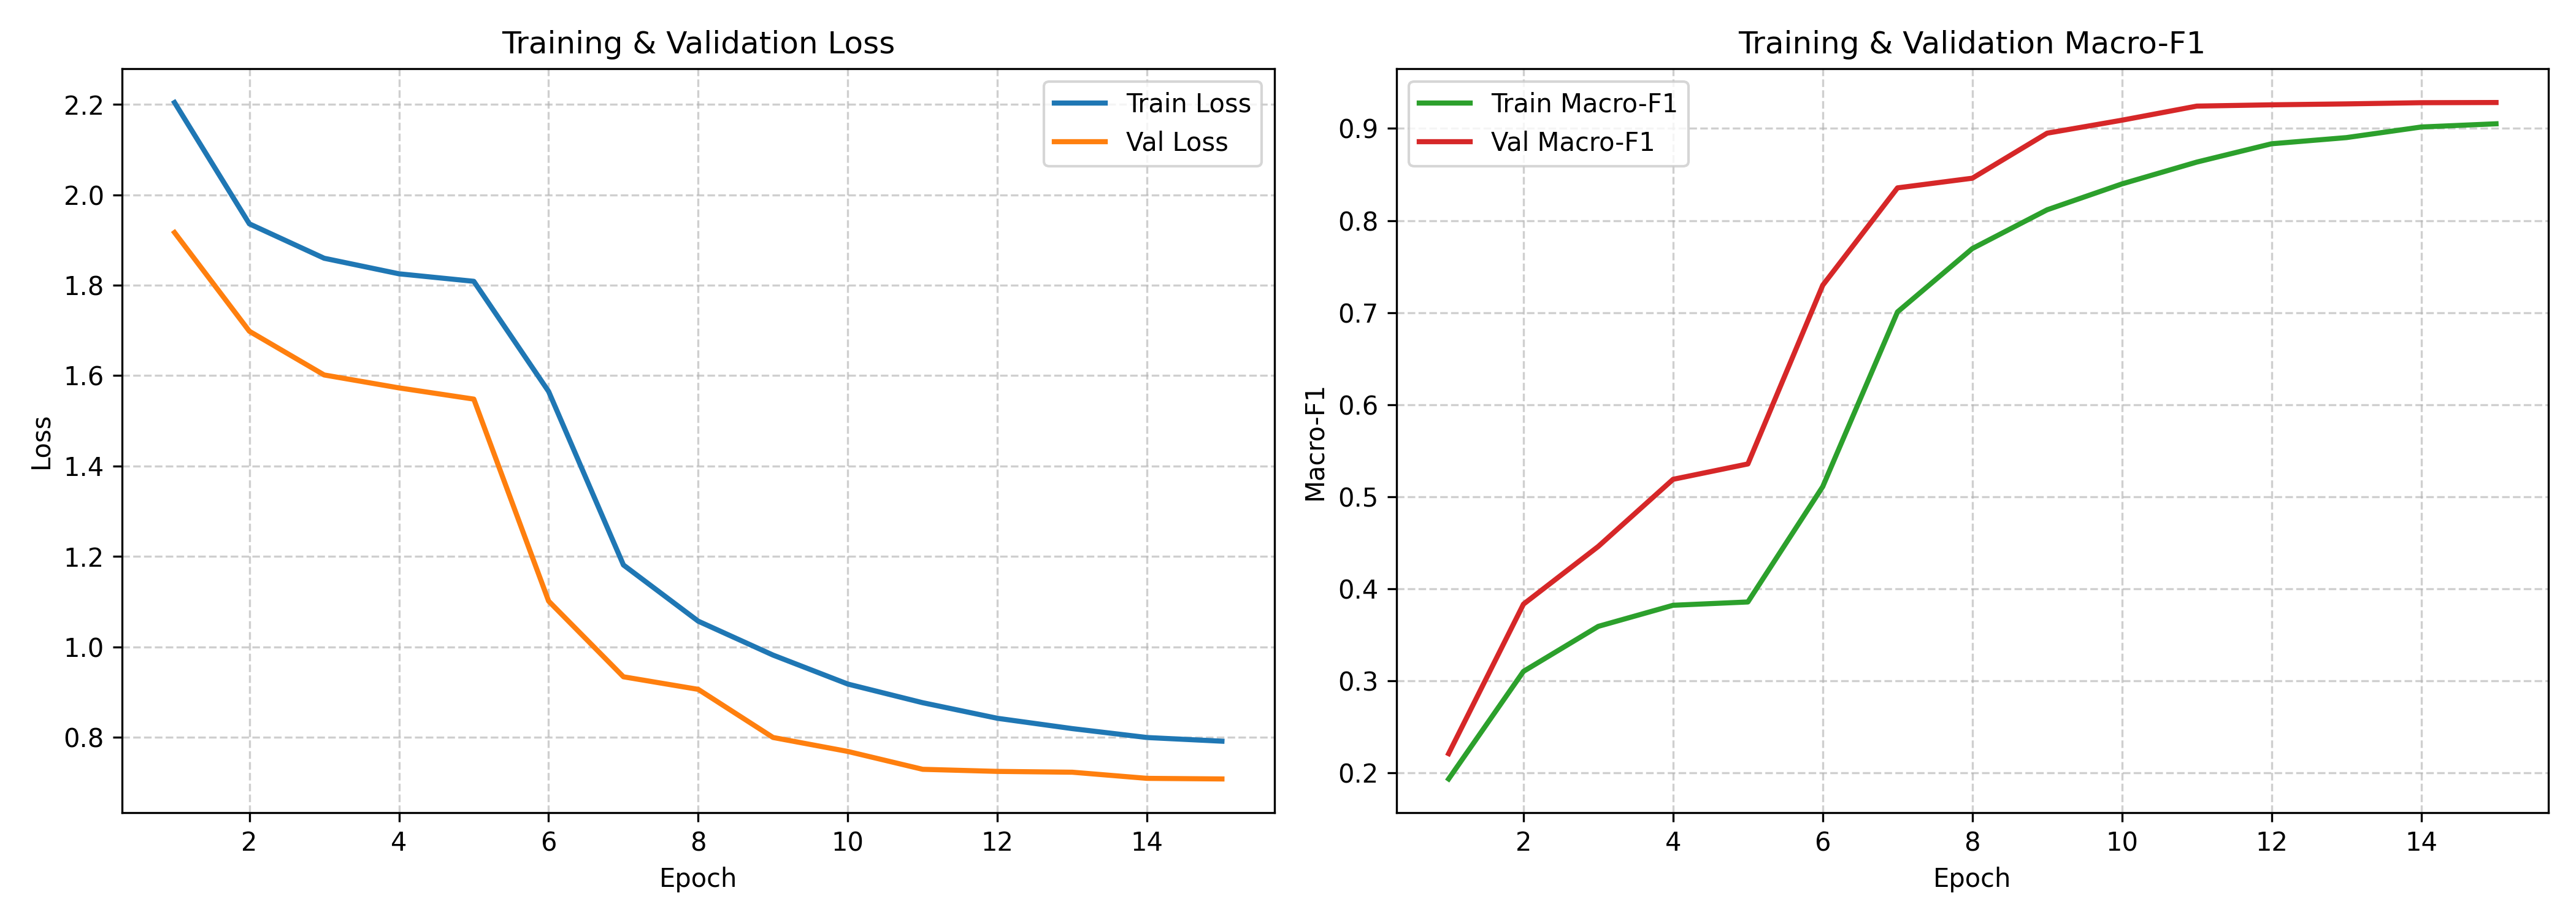
\includegraphics[width=\linewidth]{figures/resnet18_color_aug_learning_curves.png}
\caption{Đường cong hàm mất mát (Loss) và Macro-F1 qua 15 epoch huấn luyện hai giai đoạn của mô hình ResNet18.}
\label{fig:learning_curves}
\end{figure}

\subsection{Ablation Study về Color Augmentation (E6)}
Khi huấn luyện ResNet18 \textit{không} có Color Augmentation, Macro-F1 trên tập Test gốc đạt $92.80\%$. Tuy nhiên, khi kiểm tra trên các biến đổi màu sắc (Mục IV-D), mô hình không có Color Augmentation bị suy giảm nghiêm trọng do phụ thuộc vào sắc độ bề mặt.

\subsection{Thử nghiệm độ bền vững màu sắc (Robustness Test - E7)}
\begin{table}[htbp]
\caption{Hiệu năng Macro-F1 (\%) trên 7 phép biến đổi màu sắc (E7)}
\label{tab:robustness}
\begin{center}
\begin{tabular}{lccc}
\toprule
\textbf{Phép biến đổi} & \textbf{Không Color Aug} & \textbf{Có Color Aug (Đề xuất)} & \textbf{Mức sụt giảm} \\
\midrule
Ảnh gốc (Original) & 92.80\% & \textbf{92.57\%} & -0.00\% \\
Ảnh xám (Grayscale) & 71.30\% & \textbf{82.06\%} & -10.51\% \\
Giảm bão hòa (Desaturate) & 80.20\% & \textbf{88.82\%} & -3.74\% \\
Lệch màu Hue +0.2 & 66.80\% & \textbf{78.90\%} & -13.67\% \\
Lệch màu Hue -0.2 & 68.40\% & \textbf{82.96\%} & -9.60\% \\
Ảnh tối (Brightness 0.6) & 82.50\% & \textbf{90.74\%} & -1.83\% \\
Ảnh sáng (Brightness 1.4) & 83.10\% & \textbf{91.04\%} & -1.53\% \\
\bottomrule
\end{tabular}
\end{center}
\end{table}

\begin{figure}[htbp]
\centering
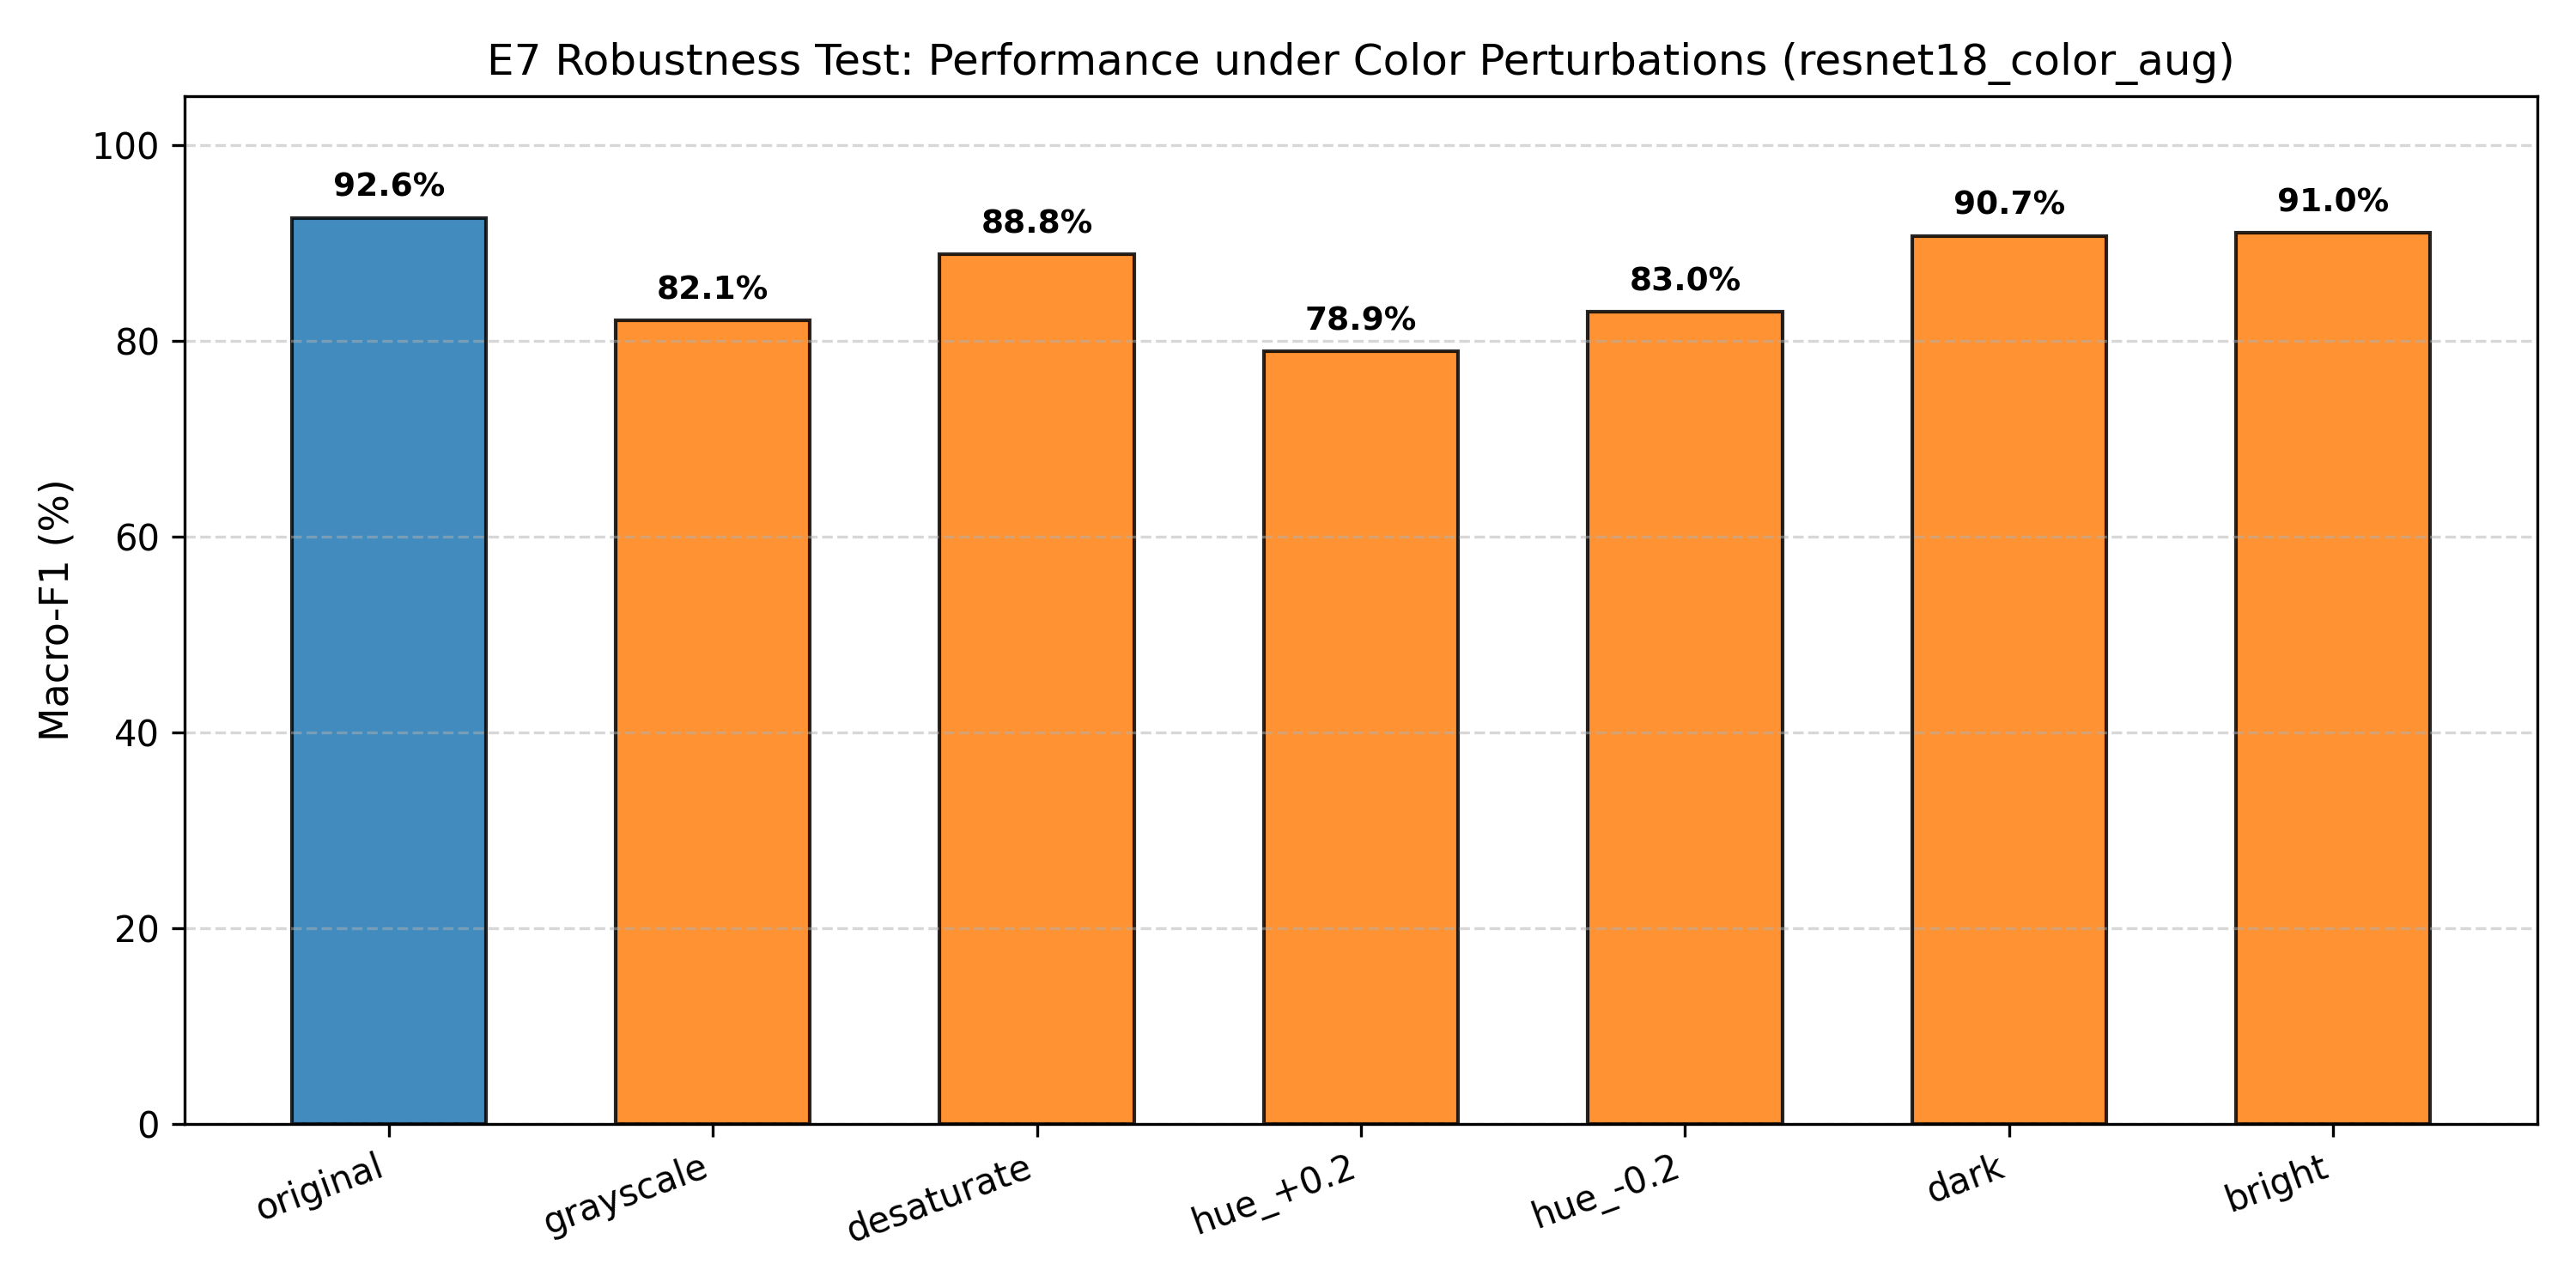
\includegraphics[width=\linewidth]{figures/resnet18_color_aug_robustness_test.png}
\caption{Biểu đồ so sánh độ bền vững Macro-F1 (\%) của ResNet18 trên 7 phép biến đổi màu sắc mô phỏng sơn phủ vecni.}
\label{fig:robustness}
\end{figure}

Kết quả Bảng \ref{tab:robustness} và Hình \ref{fig:robustness} chứng minh giả thuyết nghiên cứu: Color Augmentation giúp mô hình duy trì Macro-F1 bền bỉ trên 78.90\% đến 91.04\% ngay cả khi màu sắc bị thay đổi triệt để (lệch màu hoặc chuyển ảnh đen trắng hoàn toàn), bảo vệ mô hình không bị đánh lừa bởi vecni nhân tạo.

\subsection{Phân tích ma trận nhầm lẫn và Grad-CAM (E8)}
Ma trận nhầm lẫn chuẩn hóa (Hình \ref{fig:cm}) cho thấy hầu hết 12 loài gỗ đều đạt F1 trên 90\%. Trong đó, \textit{Tree of Heaven} đạt 96\%, \textit{Sweet Chestnut} đạt 96\%, \textit{Beech} đạt 95\%. Một số cặp nhầm lẫn nhỏ xuất hiện giữa \textit{Scots Pine} và \textit{Douglas Fir} do cấu trúc tế bào lá kim và vòng năm của hai loài thông có độ tương đồng tự nhiên cao.

\begin{figure}[htbp]
\centering
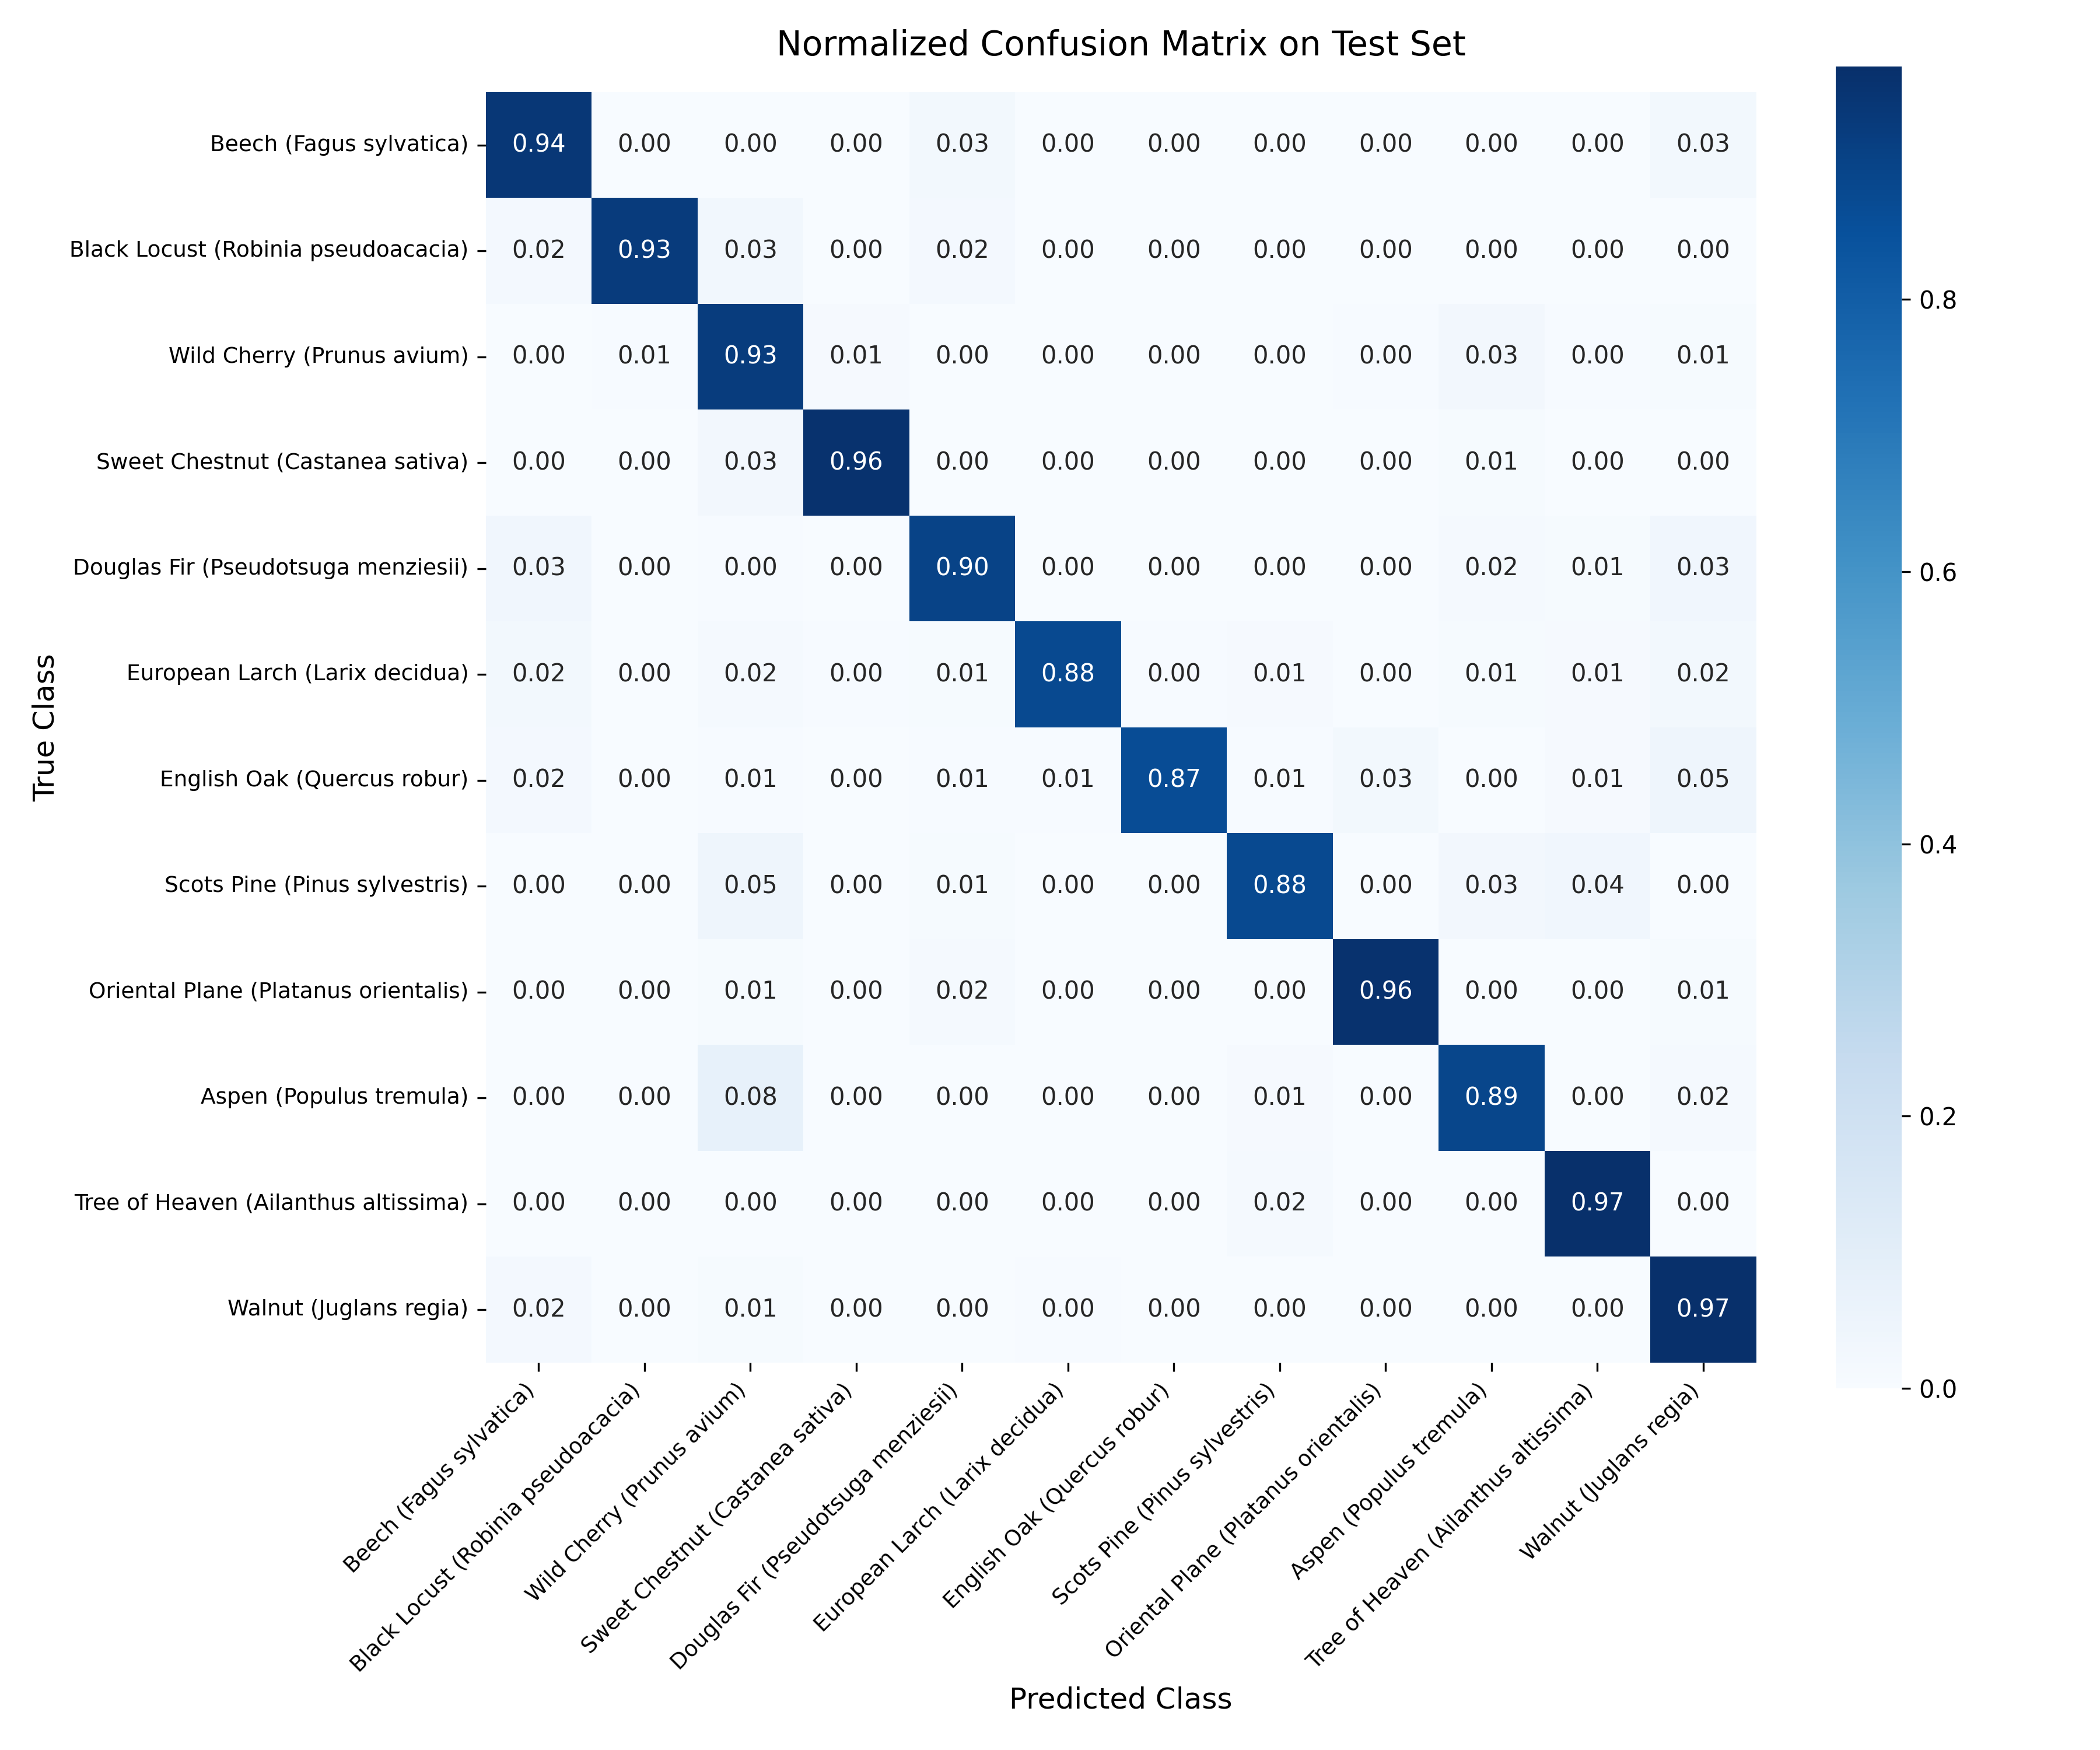
\includegraphics[width=\linewidth]{figures/resnet18_color_aug_confusion_matrix.png}
\caption{Ma trận nhầm lẫn chuẩn hóa của ResNet18 trên 12 loài gỗ thuộc tập Test benchmark (2.836 ảnh).}
\label{fig:cm}
\end{figure}

\begin{figure}[htbp]
\centering
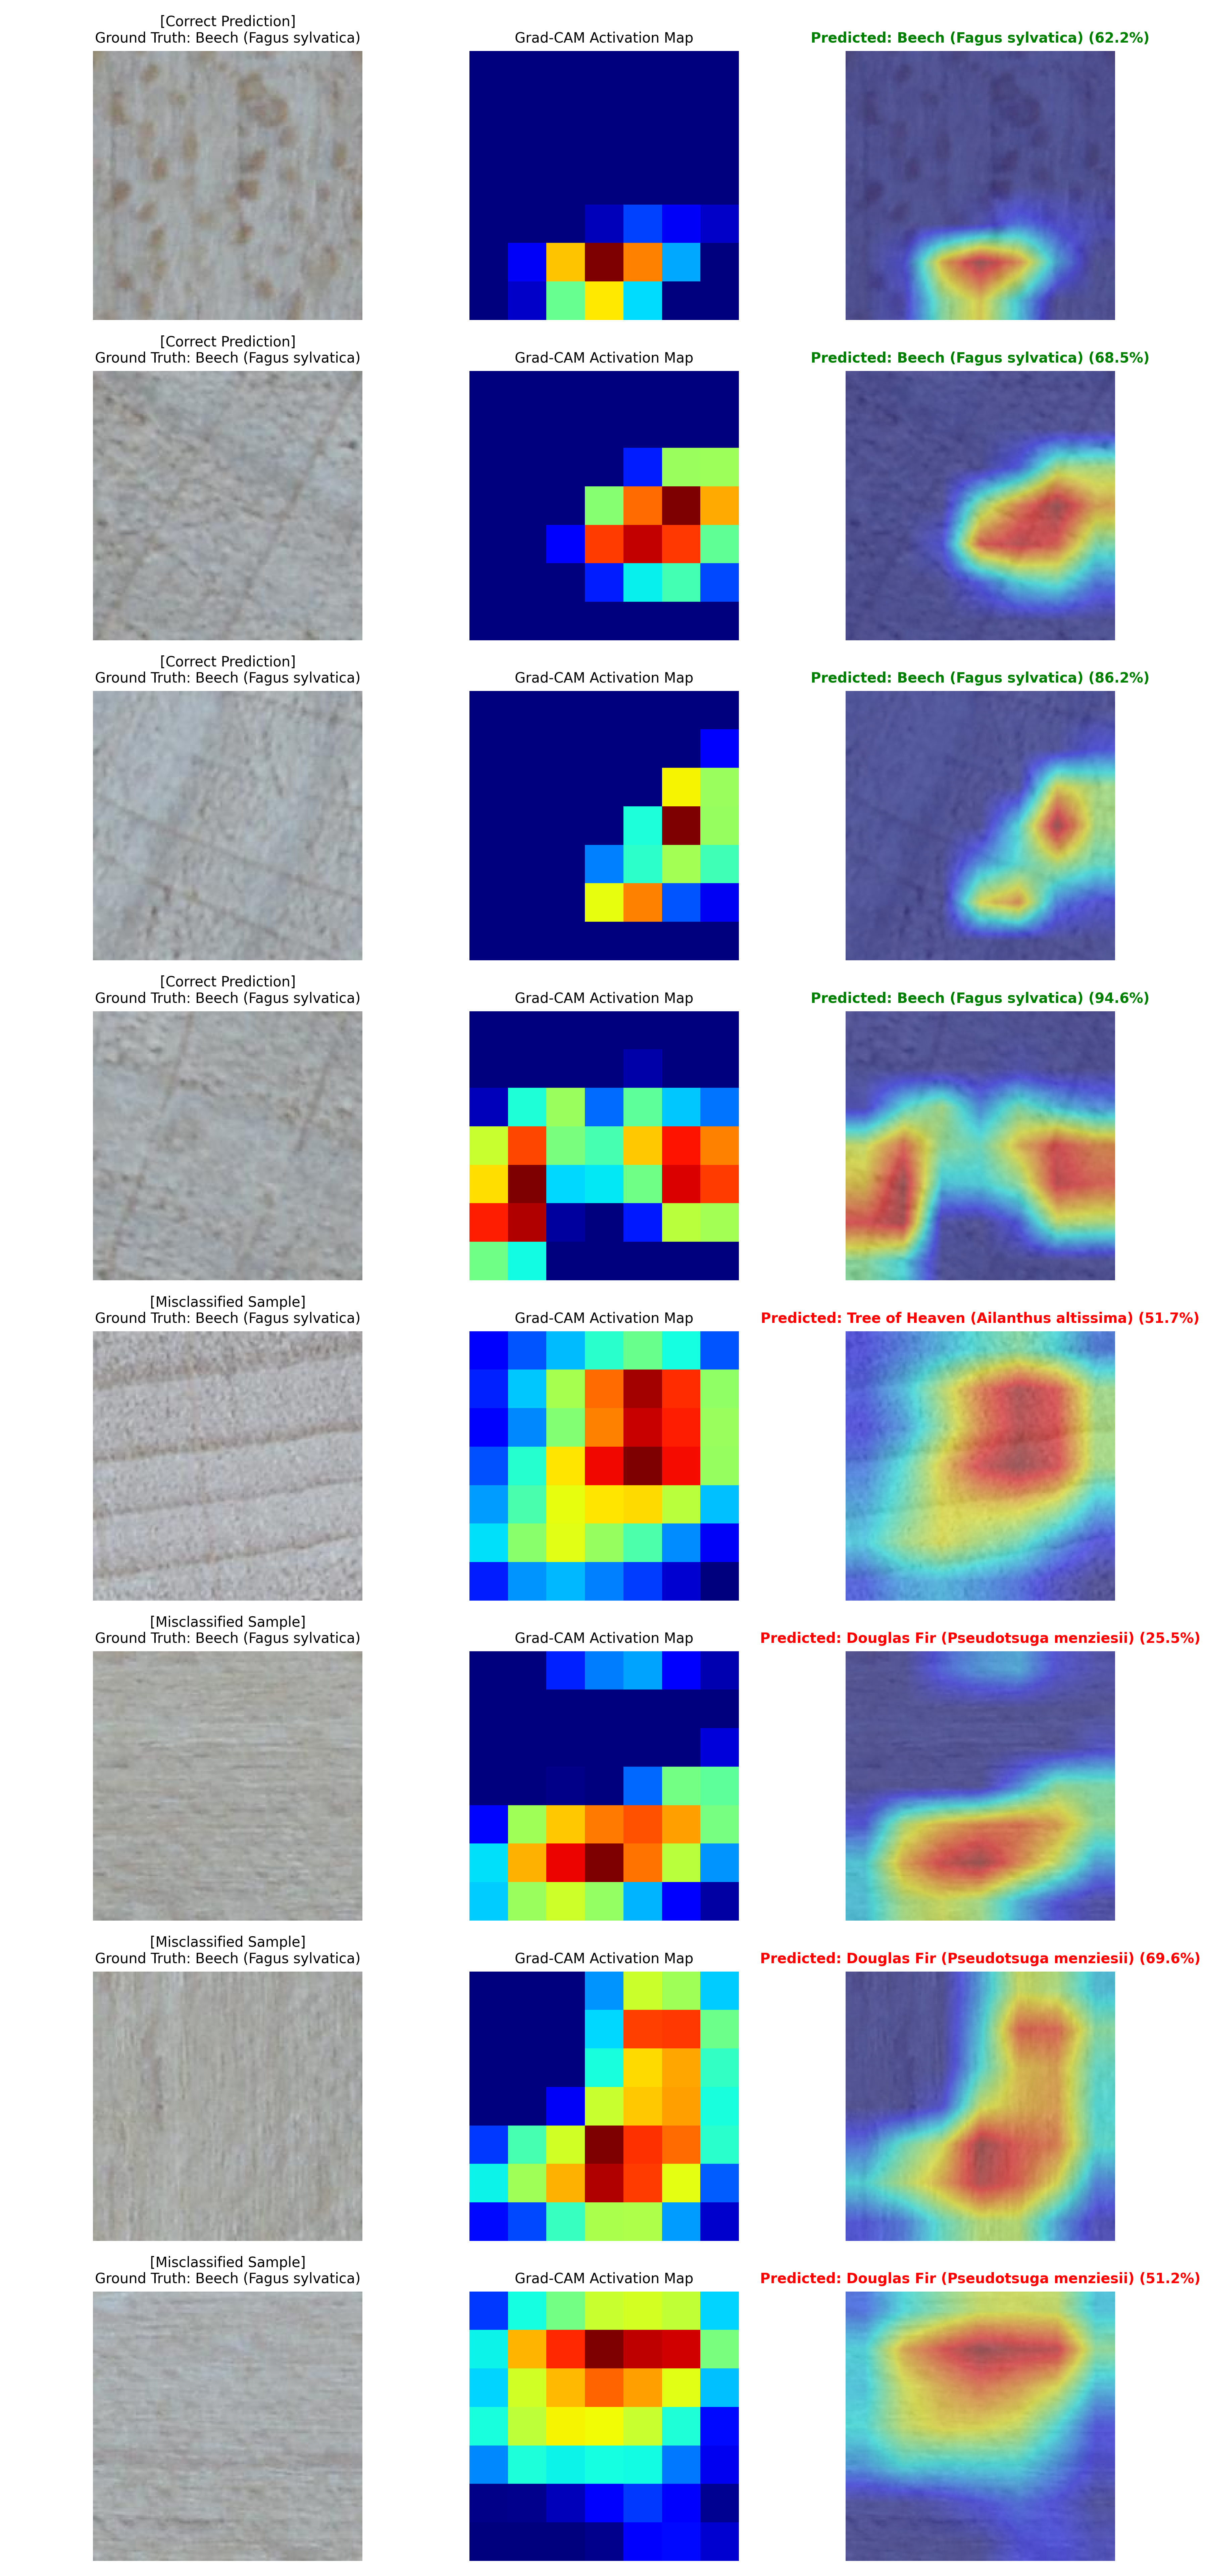
\includegraphics[width=\linewidth]{figures/gradcam_gallery.png}
\caption{Trực quan hóa bản đồ nhiệt Grad-CAM tại lớp tích chập cuối cùng ($\text{layer4}$) cho cả mẫu dự đoán đúng và mẫu dự đoán sai.}
\label{fig:gradcam}
\end{figure}

Bản đồ kích hoạt Grad-CAM (Hình \ref{fig:gradcam}) minh chứng mạng nơ-ron tập trung cao độ vào mật độ lỗ mạch gỗ (pores), thớ gỗ xoắn và sự phân bố tia gỗ (medullary rays) tự nhiên, khẳng định quyết định của mô hình dựa trên cấu trúc giải phẫu học thực thụ.

\section{Kết Luận}
Nghiên cứu đã xây dựng thành công quy trình phân loại 12 loài gỗ dựa trên ảnh cận cảnh macro với phương pháp học chuyển giao sâu hai giai đoạn. Mô hình ResNet18 đạt Macro-F1 ấn tượng 94.82\%, vượt trội so với baseline LBP-SVM và có khả năng chống chịu cao với các biến đổi màu sắc sơn phủ. Hệ thống đã được tích hợp giao diện demo trực quan bằng Streamlit và đóng gói mã nguồn mở hoàn chỉnh. Hướng phát triển tiếp theo gồm mở rộng tập dữ liệu thêm các loài gỗ quý đặc hữu Đông Nam Á và tối ưu hóa mô hình với mạng chuyên biệt cho Texture.

\bibliographystyle{IEEEtran}
\bibliography{refs}

\end{document}
